\documentclass{beamer}
\usepackage[english]{babel}
\usepackage{graphicx}
\usepackage{hyperref}

\setbeamertemplate{navigation symbols}{}

\title[PL3GA Visualisation]{Visualising the Projective Geometric Algebra of Lines}
\subtitle{Midterm Presentation}
\author{Patrick de Kok}
\institute{Supervisor: Leo Dorst}
\date{June 28, 2012}

\newcommand{\V}[1]{\ensuremath{\mathbf{#1}}}
\newcommand{\supcite}[1]{\textsuperscript{\cite{#1}}}
\newcommand{\pro}{\structure{\textbf{+}}&}
\newcommand{\con}{\structure{\textbf{--}}&}

\begin{document}
\begin{frame}
  \titlepage
\end{frame}

\begin{frame}{Project description}
    Extend a \alert<3>{graphical calculator} of \alert<1>{geometric algebra} to model the \alert<2>{projective geometry of lines}.

    \only<+>{
      \begin{itemize}
        \item Much like linear algebra, but uses more geometrically intuitive operators
        \item Outer product $\wedge$ to create subspaces
        \item Implementations are fast~\supcite{Fontijne2003}
      \end{itemize}
    }
    \only<+>{
      \begin{itemize}
        \item Useful for computer vision, graphics, robotics\ldots
        \item Pl\"ucker coordinates: 3D lines are 6D null vectors
          \begin{itemize}
            \item Representation is homogeneous
          \end{itemize}
        \item Recently found to work in geometric algebra~\supcite{Hongbo}
      \end{itemize}
    }
    \only<+>{
      \begin{center}
        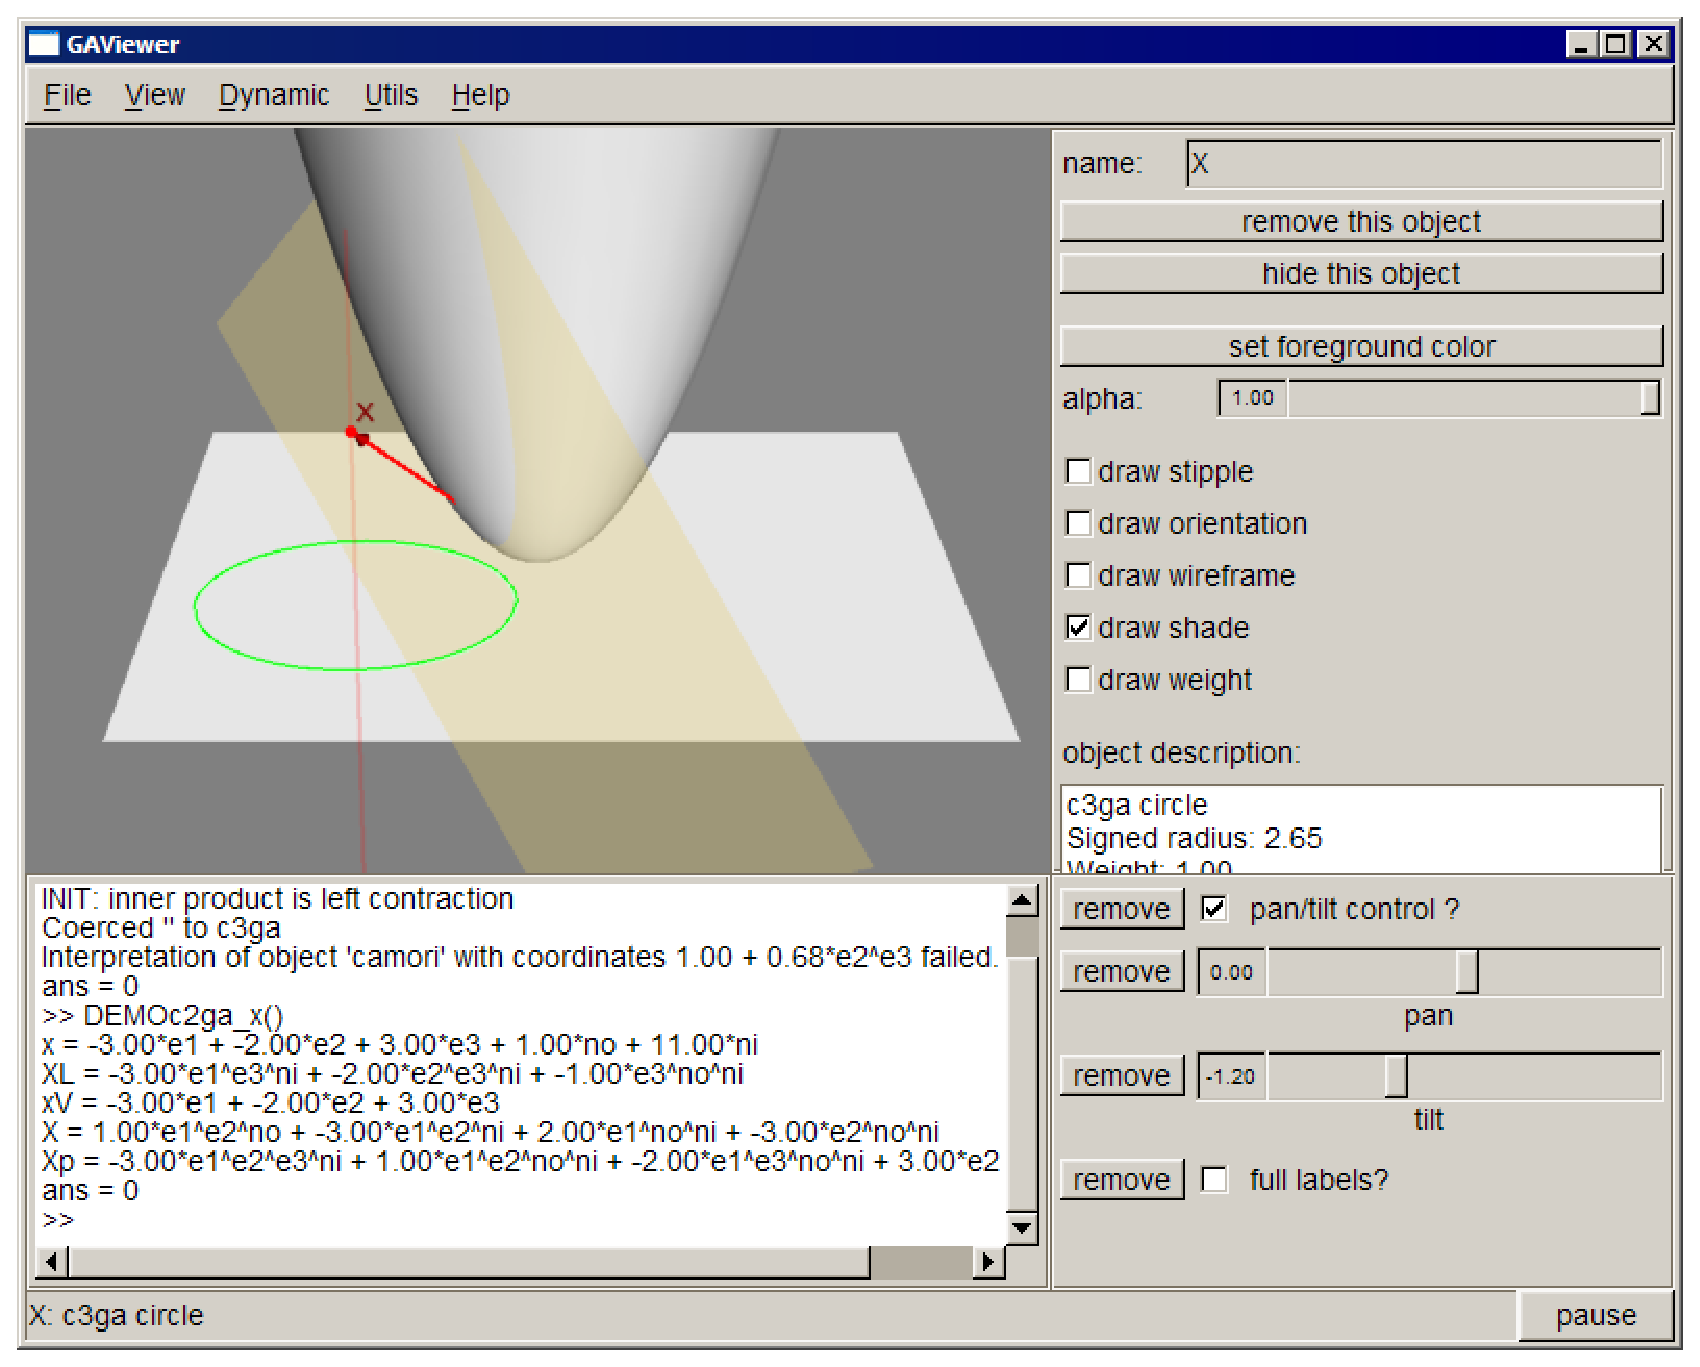
\includegraphics[width=0.7\textwidth]{gaviewer}

        \href{http://geometricalgebra.net/gaviewer_download.net}{\texttt{http://geometricalgebra.net} $\to$ Downloads $\to$ GAViewer}
      \end{center}
    }
\end{frame}

\begin{frame}{Approach}
  \begin{enumerate}
    \item Understand Pl\"ucker model for GA
    \item Compute geometric interpretation
      \begin{itemize}
        \item First by hand, then find generic formula
      \end{itemize}
    \item Extend GAViewer
      \begin{itemize}
        \item Recognise geometric type of input
        \item Computer characteristics (orientation, center, normal\ldots)
        \item Implement drawing routines
      \end{itemize}
  \end{enumerate}
\end{frame}

\begin{frame}{Projective model}
  Pl\"ucker model is really new in GA community
  \begin{itemize}
    \item Original article is badly written
    \item Must translate from text on other algebras
      \begin{itemize}
        \item Relate different inner products, $\times$ with $\wedge$
      \end{itemize}
    \item Big difference in vocabulary
    \item Some concepts not well defined
  \end{itemize}
\end{frame}

\begin{frame}{Extending GAViewer}
  \begin{tabular}{cp{4cm}|cp{4cm}}
    \multicolumn{2}{l}{\structure{Communicating through sockets}} & \multicolumn{2}{l}{\structure{Editing original code}}\\
    \pro Can use recent libraries & \con Older GA implementation is slower \\
    \pro Socket interface is clear & \con Little documentation \\
    \con Must write own parser & \pro Parser is given \\
    \con Express every element in terms of (sets of) other algebra's elements & \pro Can define completely new shapes \\
    \con End product looks ugly & \pro Final version is easier to use \\
    \con Synchronise \texttt{dynamic} variables is difficult & \pro User interaction is given
  \end{tabular}
\end{frame}

\begin{frame}{Current status}
  Done:
  \begin{itemize}
    \item Found all spots to add own code
    \item Added support for 1D, 2D subspaces, and duals
    \item All objects can be dragged (translation or rotation)
    \item Casting from and to other algebras
  \end{itemize}

  To do:
  \begin{itemize}
    \item Remove last abnormalities from 2D subspaces
    \item Add support for 3D subspaces
    \item Add support for direct representation of 4D, 5D subspaces
  \end{itemize}
\end{frame}

\begin{frame}{Questions}
  \begin{center}
    %{\Large\structure{Questions}}
    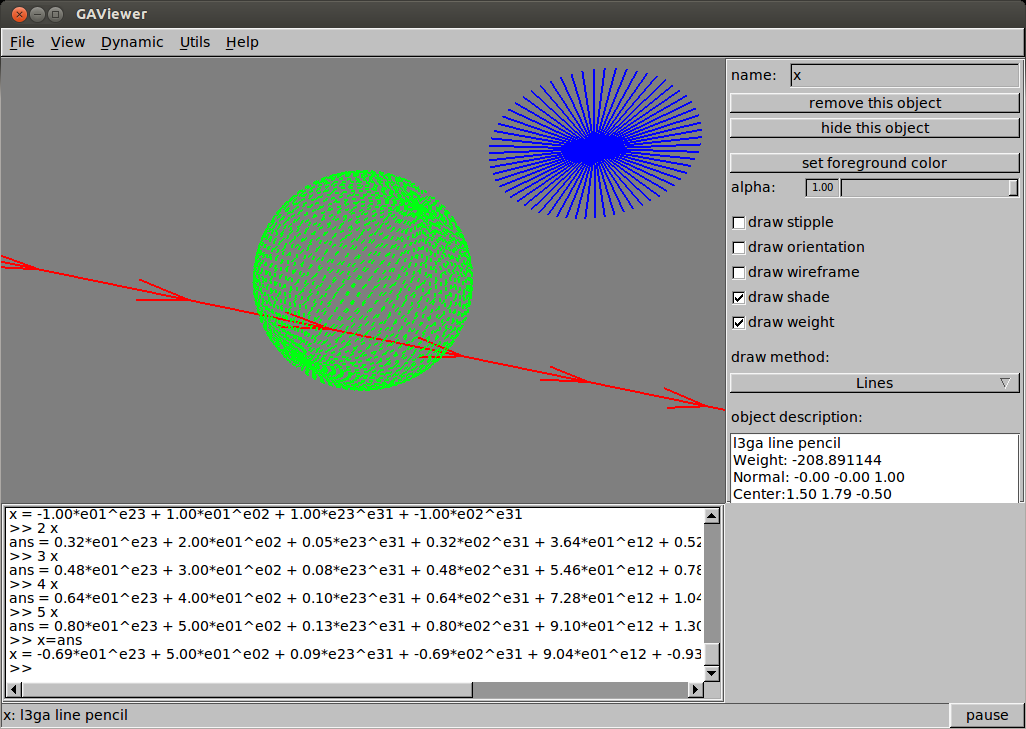
\includegraphics[width=1\textwidth]{gaviewer2}
  \end{center}
\end{frame}

\begin{frame}{Bibliography}
  \bibliographystyle{plainnat}
  \bibliography{../thesis/citations}
\end{frame}

\end{document}
